\documentclass[hyperref]{ctexart}
\usepackage[left=2.50cm, right=2.50cm, top=2.50cm, bottom=2.50cm]{geometry} %页边距
\usepackage{helvet}
\usepackage{amsmath, amsfonts, amssymb} % 数学公式、符号
\usepackage[english]{babel}
\usepackage{graphicx}   % 图片
\usepackage{url}        % 超链接
\usepackage{bm}         % 加粗方程字体
\usepackage{multirow}
\usepackage{booktabs}
\usepackage{algorithm}
\usepackage{algorithmic}
\usepackage{fancyhdr} %设置页眉、页脚
\pagestyle{fancy}
\lhead{}
\chead{}
\lfoot{}
\cfoot{}
\rfoot{}
\usepackage{hyperref} %bookmarks
\hypersetup{colorlinks, bookmarks, unicode} %unicode
\usepackage{multicol}
\title{\textbf{$\beta$ 射线的吸收}}
\author{\sffamily 赵宇航}
\date{}
\begin{document}
\maketitle
\indent{\bf 摘要: }本实验测量了铝片对$\beta$ 粒子的吸收系数,确定了 $\beta $的最大能量。 \\	
%\begin{multicols}{2}
\CTEXsetup[format={\Large\bfseries}]{section}
	\section{实验目的}
	1、了解$\beta$ 射线在物质中的吸收规律。

	2、利用吸收系数法和最大射程法,确定$\beta$ 射线的最大能量,并鉴别放射性核素。
	\section{实验原理}
	测定射线的能量是鉴別放射性核素的一种常用方法。 $\beta$射线能量的测量可用$\beta$吸收法或利用各种$\beta$谱仪直接测量$\beta$谱。本实验介绍一种最为简单的方法——$\beta$吸收法,即通过测定$\beta$粒子在吸收物质中的吸收系数或最大射程,然后换算出能量。此法求得能量的不确定性低于 5\%,目前在核燃料后处理、保健物理及污染分析等工作中有着广泛的应用。

	原子核在发生$\beta$衰变时,放出的$\beta$粒子其强度随能量变化为一条从零开始到最大能量 $E_{\beta {max}}$的连续分布曲线。一般来说,
核素的不同,其最大能量 $E_{\beta {max}}$ 不同,因此,测定$\beta$ 射线的最大能量便提供了一种鉴別放射性核素的依据。

	一束$\beta$射线通过吸收物质时,其强度随吸收层厚度増加而逐渐减弱的现象叫做$\beta$ 吸收。如图 4-1 所示,对大多数$\beta$谱,吸收曲线的开始部分在半对数坐标纸
上是一条直线,这表明它近似地服从指数衰减规律

	\begin{equation}
	I=I_0e^{-\mu d}=I_0e^{-\mu/\rho(\rho d)}=I_0e^{-\mu_md_m}\label{11}
	\end{equation}

	\eqref{11}式中$I_0$为$\beta$射线通过吸收物质前的强度;I 为$\beta$ 射线通过吸收物质后的强度;d 和$d_m$是吸收物质的厚度和质量厚度(单位分别为 cm 和 g/${cm}^2$);$\rho$为$\beta$吸收物质的密度(g/${cm}^2$);$ \mu$和$\mu_m$是线性吸收系数(${cm}^{-1}$)和质量吸收系数(${cm}^2$/g)。

	连续$\beta$谱的吸收曲线是许多单能电子吸收曲线的叠加;同时,$\beta$射线穿过吸收物质时,受到原子核的多次散射,运动方向有很大改变,因此无确定的射程可言,亦不能如同单能$\alpha$粒子的吸收那样,用平均射程来反映粒子的能量。确定$\beta$射线最大能量的方法,常用的有以下两种:

	\subsection{吸收系数法}

	实验证明,不同的吸收物质,$ \mu_m$随物质的原子序数 Z 的增加而缓慢増加。对一定的吸收物质,$ \mu_m$还与 $E_{\beta {max}}$ 有关。对于铝有下面的经验公式
	\begin{equation}
	\mu_m=\frac{17}{E^{1.14}_{\beta max}}\label{22}
	\end{equation}
其中$ \mu_m$的单位取 ${cm}^2$/g, $E_{\beta max}$ 的单位为 MeV.可见只要取吸收曲线的直线部分的数据,进行直线拟合求出$\mu_m$,并将$\mu_m$值代入(2)式,就可算出 $E_{\beta max}$ 。

	\subsection{最大射程法}

	一般用 $\beta$ 射线在吸收物质中的最大射程 $R_\beta$来代表它在该物质中的射程。因此全吸收厚度就代表$R_\beta$。通过$R_\beta$与 $E_{\beta max}$ 的经验公式或曲线即得到 $E_{\beta max}$ 。经验证明,在铝中的$R_\beta$(g/${cm}^2$)和 $E_{\beta max}$ (MeV)的关系如下:

	当 $E_{\beta max} \textgreater$0.8MeV 时($R_\beta\textgreater$0.3g/${cm}^2$),
	\begin{equation}
	E_{\beta max}=1.85 R_{\beta}+0.245
	\end{equation}

	当0.15MeV$\textless E_{\beta max}\textless$ 0.8MeV 时(0.03g/${cm}^2$$\textless R_\beta\textless$0.3g/${cm}^2$),
	\begin{equation}
	E_{\beta max}=1.92 R_{\beta}^{0.725}\label{3b}
	\end{equation}

	当$E_{\beta max}\textless$ 0.2MeV 时,
	\begin{equation}
	E_{\beta max}=1.85 R_{\beta}^{1.67}
	\end{equation}


	在这种方法中,$E_{\beta max}$ 的不确定性与$R_\beta$和射程——能量关系式的准确程度有关。实际测量中,常把计数率降到原始计数率(无吸收)万分之一处的吸收厚度作为
$R_\beta$。在测量吸收曲线时,$\beta$ 射线和轫致辐射的干扰能够使得在吸收厚度超过$R_\beta$后仍有较高的计数。例如,为原始计数率的 1\%,这就给射程的估计带来很大的误差。通常可用以下方法处理:
	1.直接外推法
将吸收曲线上各点计数,作本底和空气吸收厚度校正后,连接成一条新曲线,在新曲线上,计数率降低为原始计数率的百分之一处对应的横坐标之值(g/${cm}^2$)即为最大射程$R_\beta$。对曲线不够长,需按趋势外推到百分之一处,故此法称为直接外推法。此种处理方法,对较强的单能纯β源求得的$R_\beta$较精确,但当源较弱或同时放出两种以上$\beta$射线且有$\gamma$射线时,外推的任意性较大,因此所求得的$R_\beta$误差也较大
	\section{实验结果}
	\subsection{吸收系数法}
	前后两次本底计数的均值都在50 ,去除本底后吸收片的数量与粒子数及其误差如下表
	$$\begin{tabular}{|c|c|c|c|c|c|c|c|c|c|c|c|c|c|}
	\hline
	吸收片数量 & 0 & 1 & 2 & 3 & 4 & 5 & 6 & 7 & 8 & 9 & 10 \\ \hline
	粒子数 		& 11608 & 6072 & 3528 & 2346 & 1769 & 1479 & 1320 & 1219 & 1148 & 1086 & 1033  \\ \hline
	相对误差(\%) & 1.17 & 1.73 & 1.50 & 1.52 & 1.62 & 1.67 & 1.73 & 1.46 & 1.54 & 1.61 & 1.69	\\ \hline
	吸收片数量 & 11 & 12 & 13 & 14 & 15 & 16 & 17 & 18 & 19 & 20 &\\ \hline
	粒子数 		& 986 & 945 & 901 & 871 & 831 & 790 & 756 & 730 & 692 & 661 &   \\ \hline
	相对误差(\%) & 1.74 & 1.81 & 1.86 & 1.94 & 1.78 & 1.76 & 1.82 & 1.86 & 1.91 & 1.68 &  \\ \hline
	\end{tabular}$$

	对粒子数取对数后,半对数坐标纸上画出吸收曲线如下(实验相对误差如上表)
	\begin{figure}[H]
	\begin{minipage}{0.5\linewidth}
	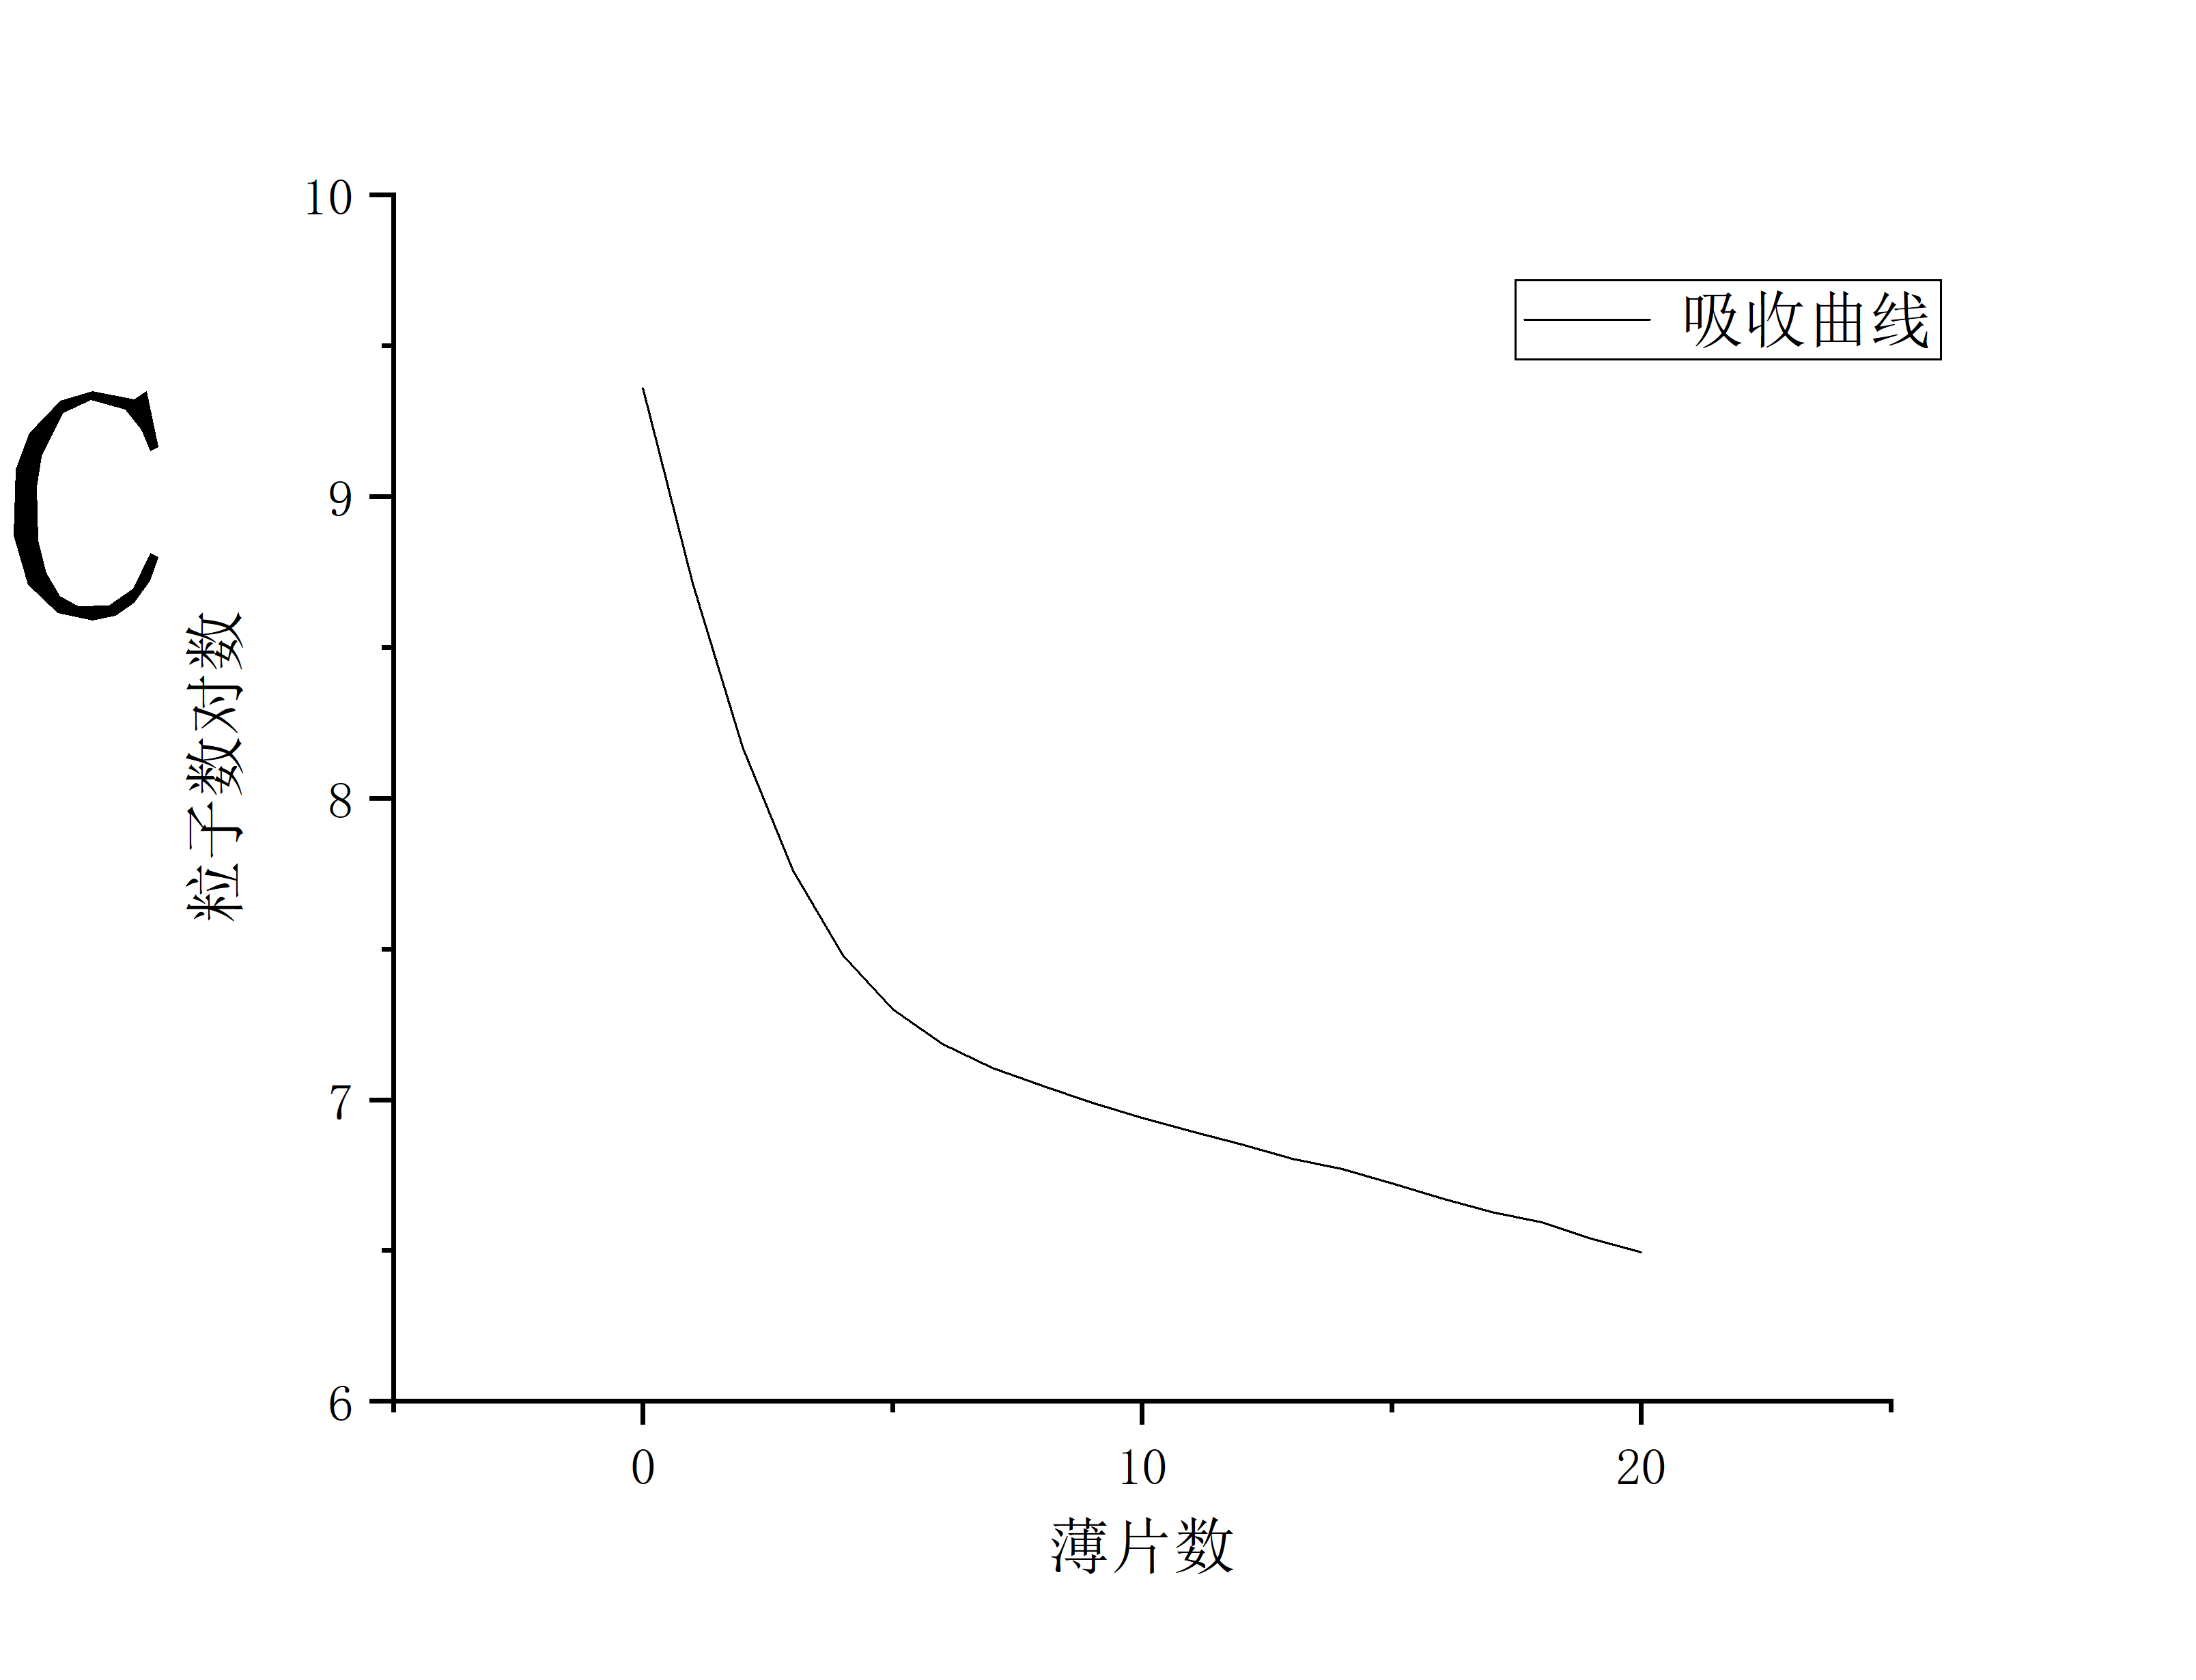
\includegraphics[scale=0.3]{t11}
	\end{minipage}
	\begin{minipage}{0.25\linewidth}
	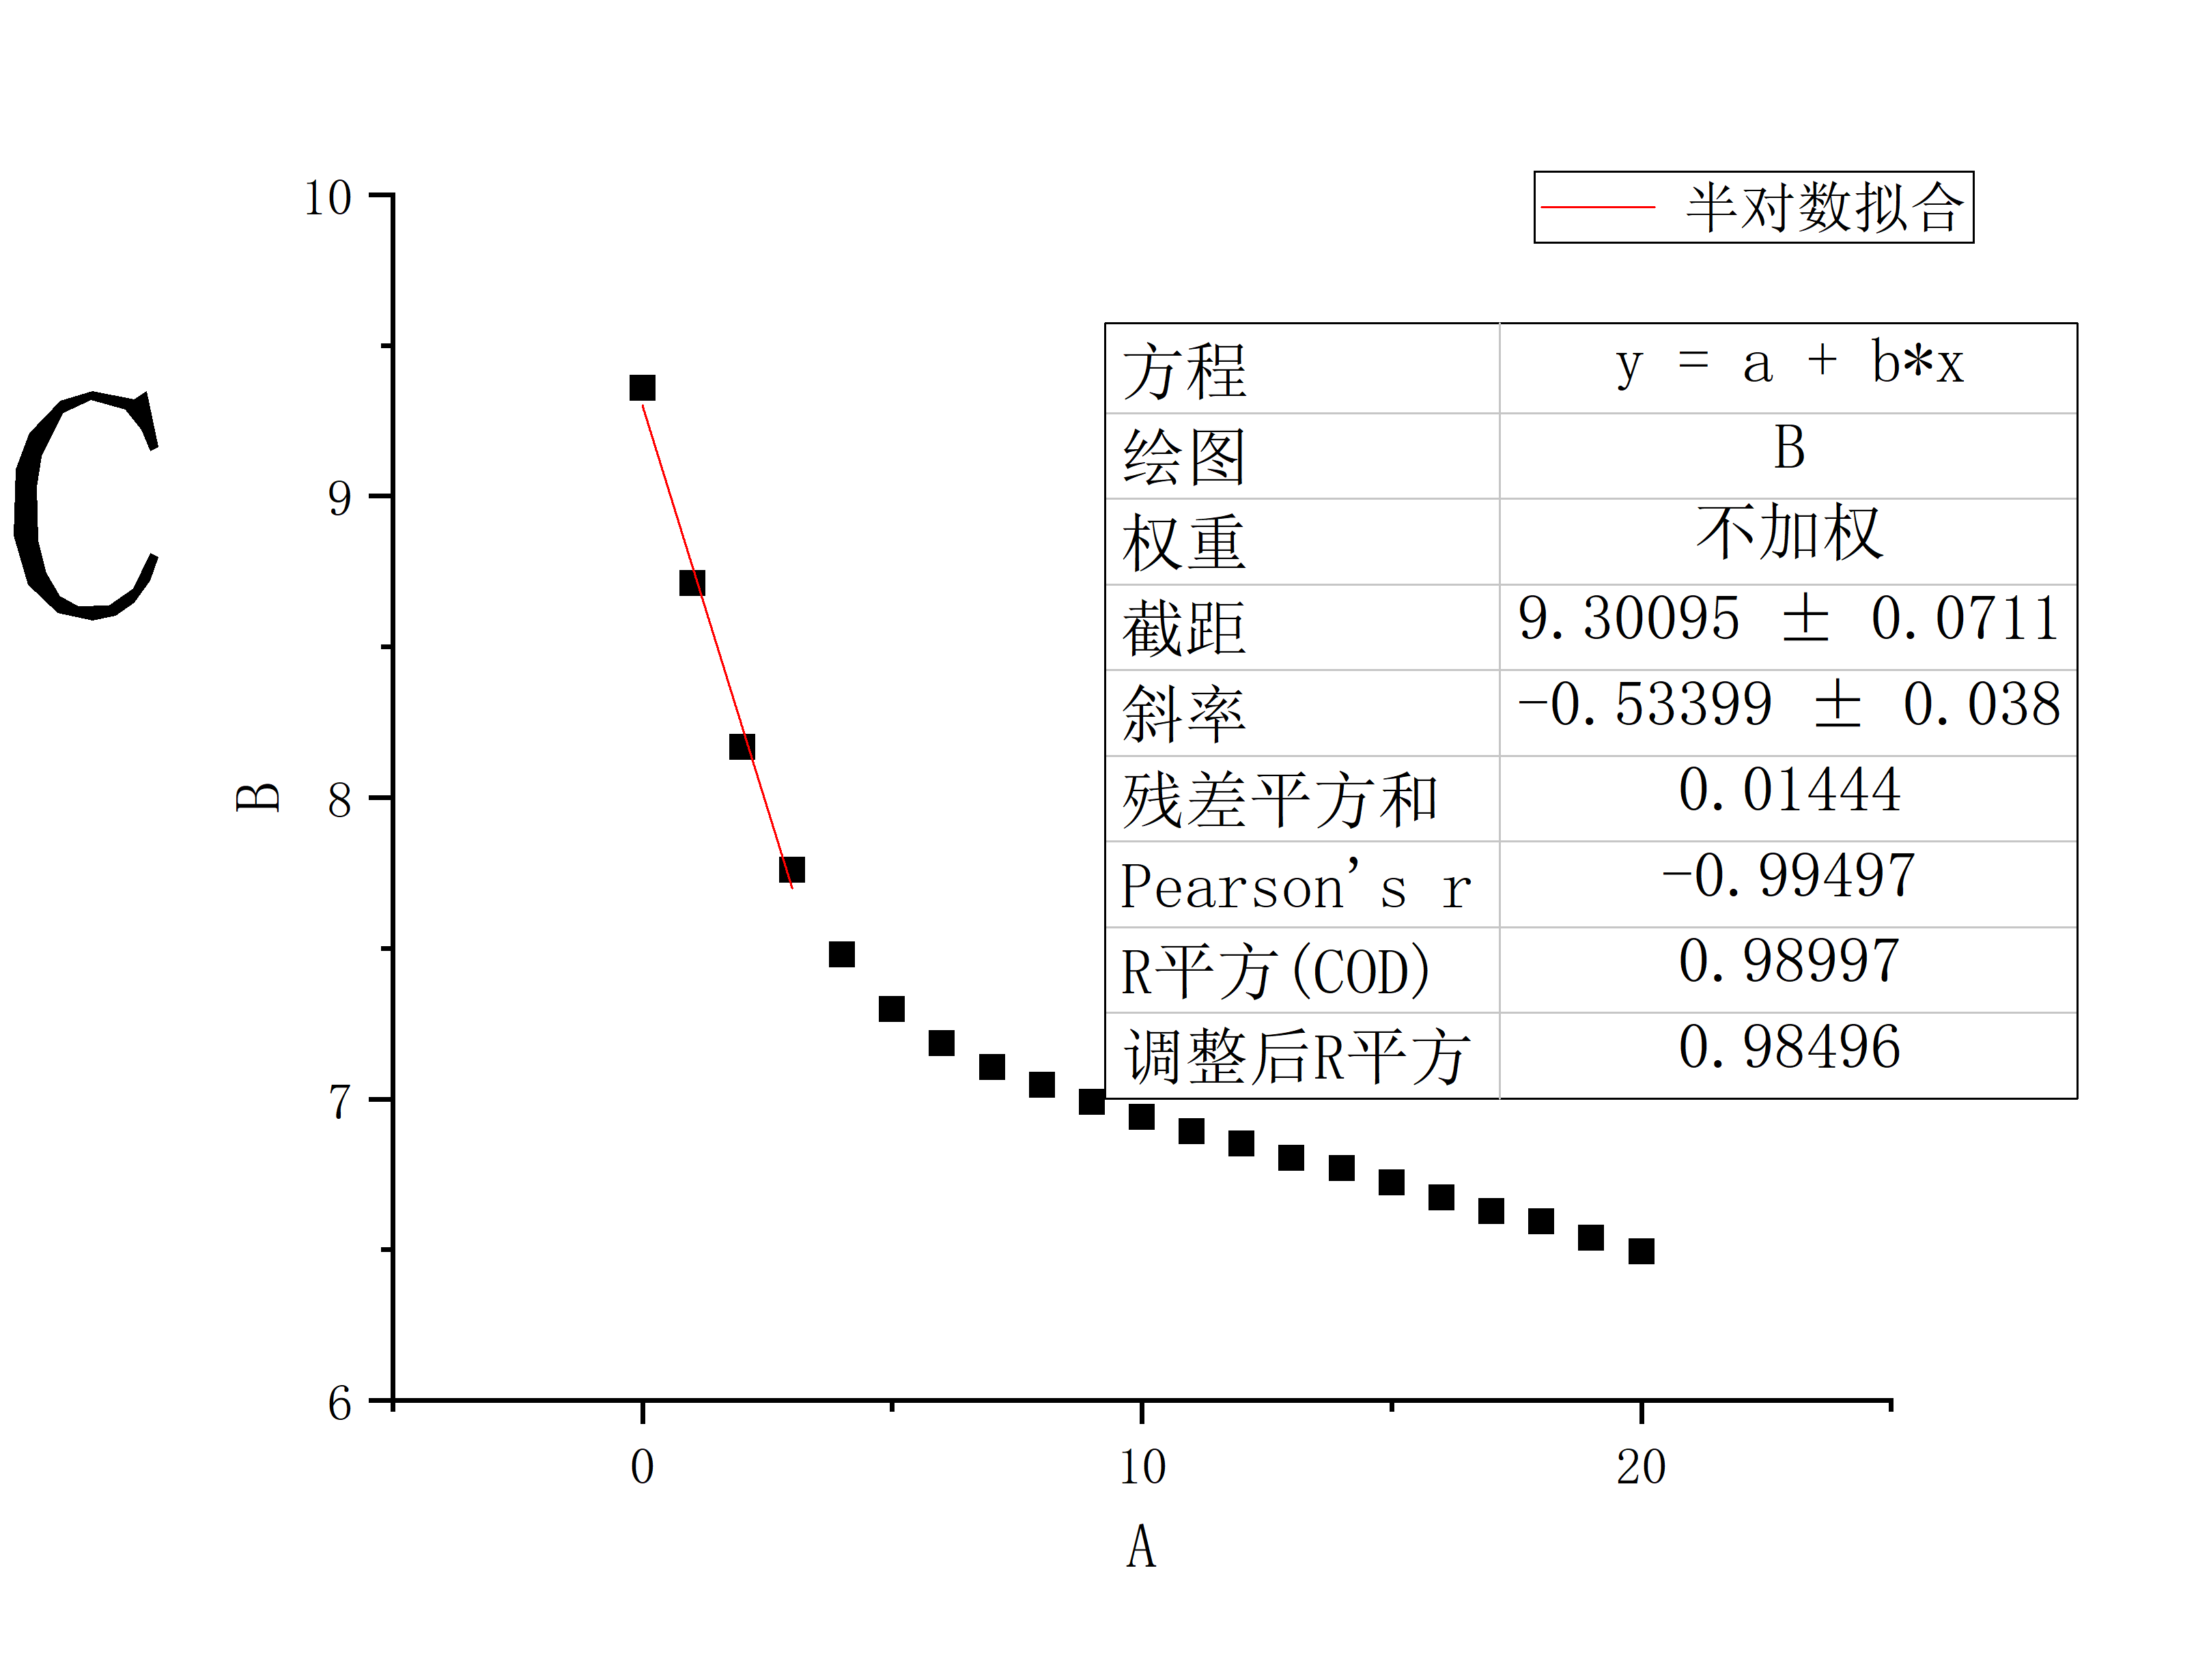
\includegraphics[scale=0.3]{t12}
	\end{minipage}
	\end{figure}
	拟合曲线如上,注意到实验中每片质量厚度为$0.02g/{cm}^2$,故$\mu_m = 26.7{cm}^2/g$。利用式\eqref{22}可以求得$E_{\beta max} = 0.673 MeV$。

	\subsection{直接外推法}
	对粒子数以10为底取对数后,画出吸收曲线如下
	\begin{center}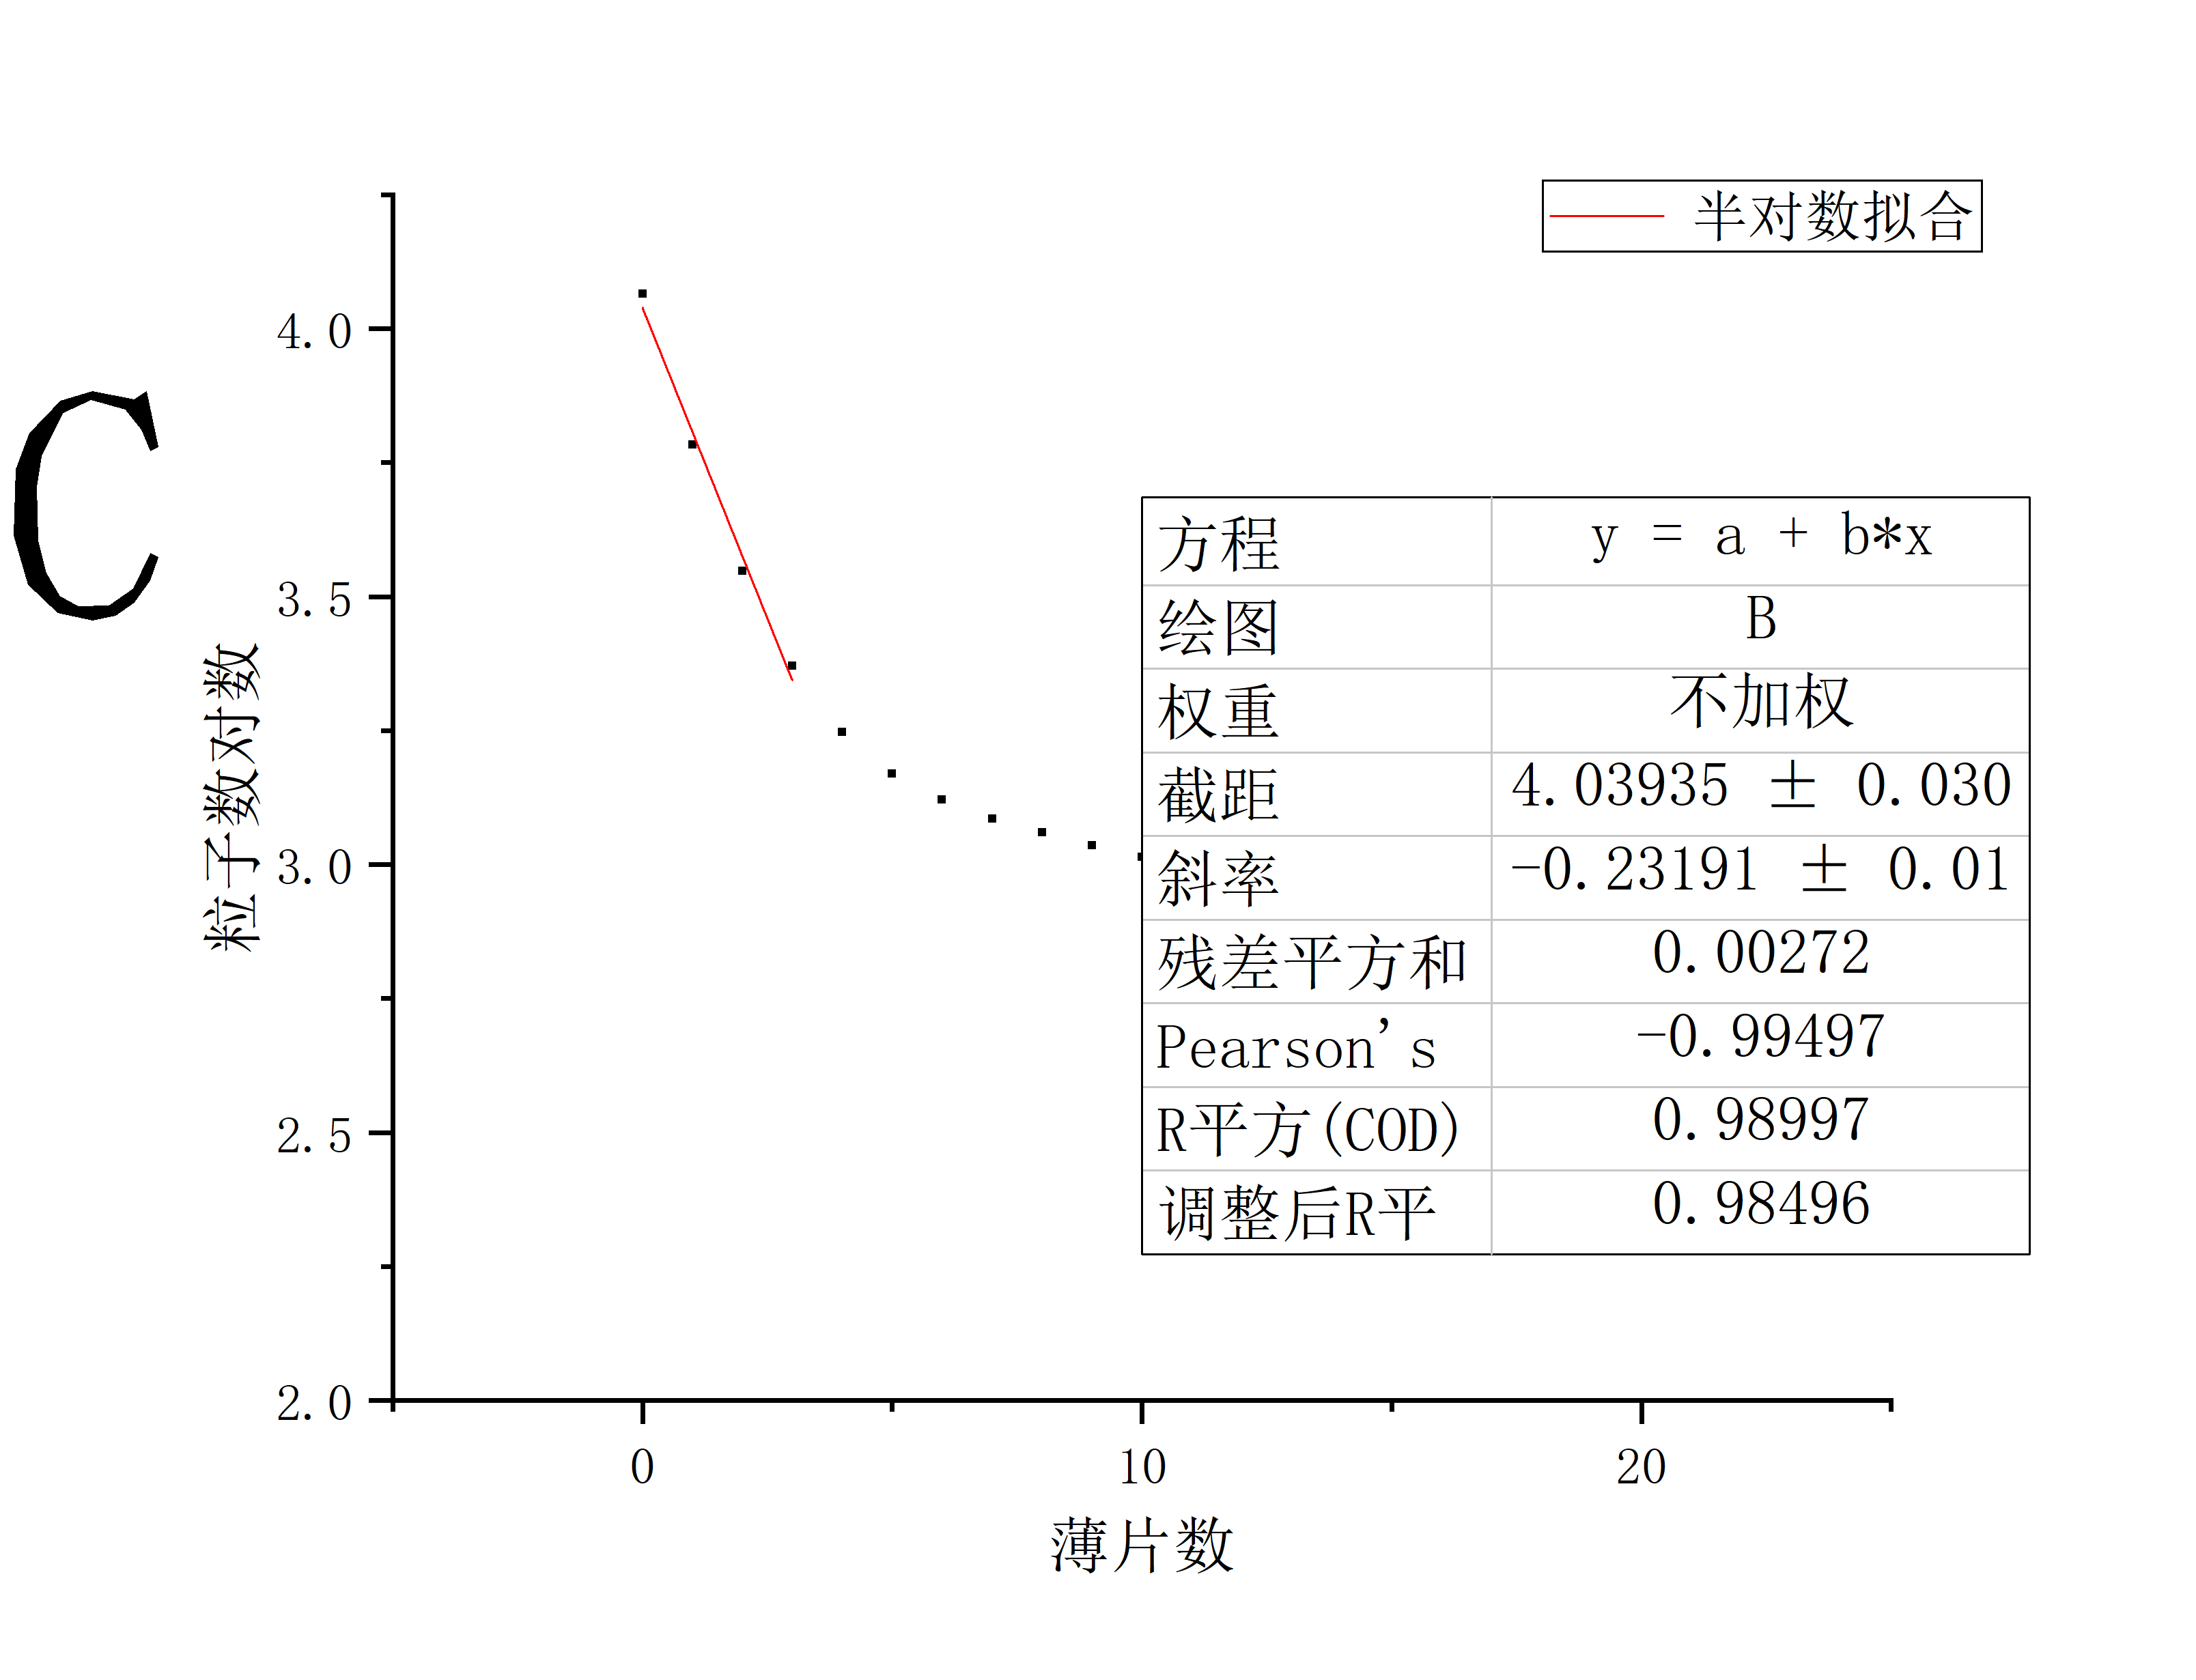
\includegraphics[scale=0.3]{t13}\end{center}
	延长后知直线与$y=2$交于$(8.87,2)$,即$R_{\beta} = 0.1774g/{cm}^2$。利用式\eqref{3b},求得$E_{\beta max} = 0.548 MeV$。

	比较知待测源为$Cs-137$,查资料知其最大$\beta$衰变的能量为0.512MeV 。相对误差为7.0\% 。

	\section{讨论}
	 内转换常在重原子的最内几个电子壳层中发生,发射$\gamma$射线,其能量较高;$\beta$射线一般会取代外层电子,能量较低。

	$\alpha$射线的穿透能力差,在空气中的射程只有1~2厘米;$\beta$射线穿透本领较强。$\alpha$粒子是带正电的重粒子,在空气中极易电离,也容易与其他粒子碰撞,所以速度降低得很快,穿透能力差。

	利用式\eqref{22}可以求得最大射程$R_{\beta} = 0.281 g/{cm}^2$。不能否用同一经验公式估计它在硅中的射程,不同元素的电子排布不同,致密程度也不同,测出来的经验曲线也不同。

	粒子被散射后,所测得粒子数减少,测得吸收系数增大。可以选择原子核比较小的元素充当吸收片减少散射的影响。

	采用较薄的吸收片,依此增加吸收片的数量,直到吸收曲线明显不成直线。因为这样测出来比较精确,也节约了一部分时间。

	吸收系数法直接通过$\mu_m$求出最大能量,需要对曲线斜率进行拟合,但总体来说比较方便。直接外推法,有三段拟合公式,拟合较为精准,但是外推的过程误差很大。


















%\end{multicols}
\end{document}